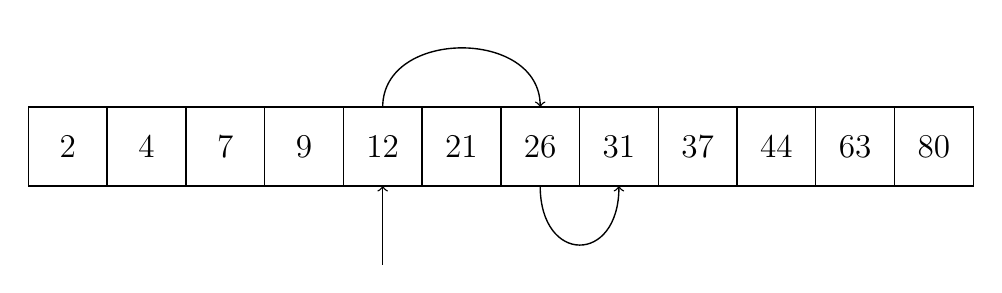
\begin{tikzpicture}[->,node distance=1cm, box/.style={draw,shape=rectangle,minimum size=1cm,font=\large},line width=0.5pt]
    \node[box] (1) at (0,0) {2};
    \node[box] (2) [right of=1] {4};
    \node[box] (3) [right of=2] {7};
    \node[box] (4) [right of=3] {9};
    \node[box] (5) [right of=4] {12};
    \node[box] (6) [right of=5] {21};
    \node[box] (7) [right of=6] {26};
    \node[box] (8) [right of=7] {31};
    \node[box] (9) [right of=8] {37};
    \node[box] (10) [right of=9] {44};
    \node[box] (11) [right of=10] {63};
    \node[box] (12) [right of=11] {80};

    \draw (4,-1.5) -- (4,-0.5);
    \draw (4,0.5) .. controls +(90:1) and +(90:1) .. (6,0.5);
    \draw (6,-0.5) .. controls +(-90:1) and +(-90:1) .. (7,-0.5);
\end{tikzpicture}
